\documentclass[../PHYS306Notes.tex]{subfiles}

\begin{document}
\section{Lecture 16}
\subsection{Lecture Notes - Focault Pendulum}
\subsubsection{Rotating Coordinate System EOM}
\[
\begin{array}{c}
\left(\frac{d \v{Q}}{d t}\right)_{S_{0}}=\left(\frac{d \v{Q}}{d t}\right)_{S}+\vec{\omega} \times \v{Q} \\
m \ddot{\v{r}}=\vec{F}+2 m \dot{\v{r}} \times \v{\Omega}+m(\v{\Omega} \times \v{r}) \times \v{\Omega}+m \v{r} \times \dot{\vec{\Omega}}=\v{F}+\v{F}_{\text {coriolis }}+\v{F}_{\text {centrifugal }}+\v{F}_{\text {Euler }}
\end{array}
\]

\subsubsection{Review Questions}
A bead rests on a wire that extends from the origin at an angle $\theta$ to the vertical. The wire rotates with angular velocity $\Omega$ about the vertical. In the frame rotating with the wire, what is the magnitude and direction of the centrifugal force when the bead is a distance $r$ from the origin?
\begin{s}
By trigonometry, the bead is $r\sin\theta$ away from the rotation axis, so there is a centrifugal force of $m\Omega^2r\sin\theta$ away from the rotation axis.
\end{s}

A bucket of water spins about its central axis. After a relaxation time, the shape of the water surface reaches a steady state. Where is the water surface highest?
\begin{s}
At the edge of the bucket, as the centrifugal force pulls the water towards the edge. The surface of the water is a parabola.
\end{s}
\begin{center}
    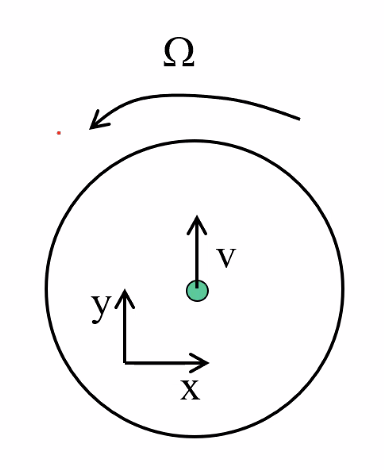
\includegraphics[scale=0.5]{Lecture-16/l16-img1.png}
\end{center}
A puck slides from the center towards the edge of a frictionless, rotating merry-go-round. The merry-go-round has angular velocity $\Omega$ and rotates CCW when viewed from above. In the rotating frame, the initial velocity is in the positive $y$ direction. What effect does the Coriolis force have on the velocity of the puck?
\begin{s}
The coriolis force changes the direction of the velocity (deflected left) but does not change the magnitude (we can see from the $\v{v} \times \v{\Omega}$ form that the force does no work).
\end{s}

Consider the same scenario as the previous question. How many rotations does the merry-go-round make before the puck slides off of the edge?

\begin{s}
$\# \text{rotations} = \frac{a\Omega}{2\pi v}$. First consider that the time to reach the edge is simply the distance $a$ (radius) divided by the velocity $v$ of the puck. Then, we may divide this time by the time per rotation (the period), which is $T = \frac{2\pi}{\Omega}$. This yields:
\[\# \text{rotations} = \frac{\Delta t}{T} = \frac{a\Omega}{2\pi v}\]
\end{s}

At which of these points will a person's measured weight be the largest (equator, 30, 40, 60 degrees latitude, or north pole)
\begin{s}
At the north pole; there we have no centrifugal force there (which acts against the gravitational force and decreases the weight of the person). 
\end{s}

In the northern hemisphere, which directions are winds from the north and south deflected by the Coriolis force?
\begin{s}
Winds from the N are deflected E and winds from the S are deflected W.
\end{s}

Where are these low pressure areas?
\begin{center}
    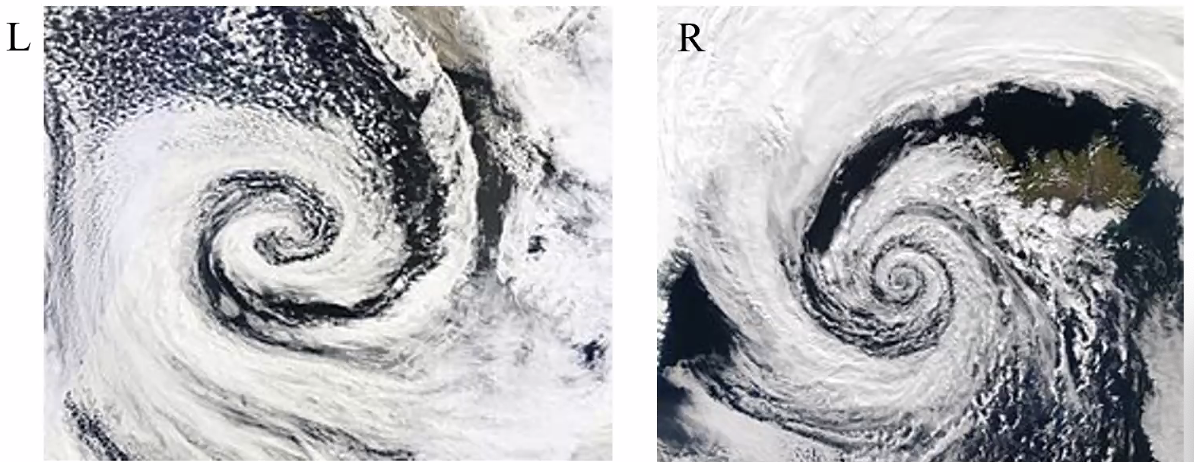
\includegraphics[scale=0.5]{Lecture-16/l16-img2.png}
\end{center}
\begin{s}
The left image rotates clockwise, the right one rotates counterclockwise. For a low pressure system, we have air coming in, and in the northern hemisphere, we have right deflection (and vise versa for the southern hemisphere) so we would expect a counterclockwise motion for the northern hemisphere and clockwise for the southern hemisphere.
\end{s}

\subsubsection{The Foucault Pendulum}
We start with our general expression:
\[m\ddot{\v{r}} = \v{F} + 2m\dot{\v{r}}\times \v{\Omega} + m(\v{\Omega} \times \v{r})\times \v{\Omega} + m\v{r}\times \dot{\v{\Omega}}\]
The third term can be neglected as the Earth spins at a constant rate, and the second term can be neglected as $\Omega$ is small. Define $x$ to be north south, $y$ to be east west. $\v{F}$ is the sum of the tension and the gravitational force, that is:
\[\v{F} = \v{T} + m\v{g}\]
Now we consider the given picture:
\begin{center}
    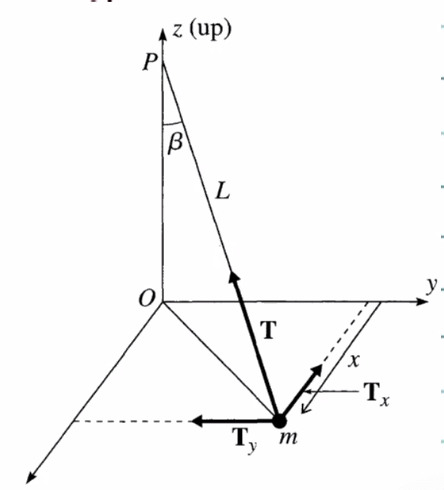
\includegraphics[scale=0.5]{Lecture-16/l16-img4.png}
\end{center}
By similar triangles:
\[T_x = -T\frac{x}{L}\]
\[T_y = -T\frac{y}{L}\]
\[T_z = -T\frac{z-L}{L}\]
But for the $T_z$, we can consider that we do small amplitudes, so $z \approx 0$, and $\dot{z} \approx 0$. Hence, $T_z \approx T \approx mg$. Hence, we have dealt with the tension. Now, we think about $\v{\Omega}$.
\begin{center}
    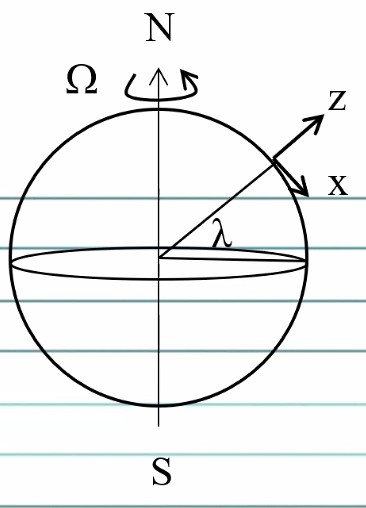
\includegraphics[scale=0.5]{Lecture-16/l16-img3.png}
\end{center}
If our latitude is $\lambda$ and we use coordinates such that $x$ points towards the equator, $y$ points parallel to the latitude line, and $z$ points away from the center of the earth, what is the rotation vector in this coordinate system?
\begin{s}
We know that $\v{\Omega}_{earth}$ points straight upwards. Projecting this, we get:
\[\v{\Omega} = \omega\m{-\cos\lambda \\ 0 \\ \sin\lambda}\]
\end{s}
Next, what is $\v{\Omega} \times \v{v}$?
\begin{s}
Using that $\v{v} = \m{\dot{x} \\ \dot{y} \\ 0}$ (Assume $\dot{z}$ is negligible) and $\v{\Omega}$ from above, we get:
\[\v{\Omega} \times \v{v} = \m{-\dot{y}\Omega \sin\lambda \\ \dot{x}\Omega\sin\lambda \\ -\dot{y}\Omega\cos\lambda}\]
\end{s}
Now, putting together the equations of motion for $x$ and $y$ we get:
\[m\ddot{x} = -mg\frac{x}{L} + 2m\Omega\sin\lambda \dot{y}\]
\[m\ddot{y} = -mg\frac{y}{L} - 2m\Omega\sin\lambda\dot{x}\]
We have a system of coupled equations. As a trick, multiply both equations by $i$ and add them together, and define $s = x + iy$. We then have:
\[\ddot{s} + 2i\alpha \dot{s} + k^2\dot{s} = 0\]
Where $\alpha = \Omega\sin\lambda$, $k^2 = \frac{g}{L}$. To solve this differential equation, we guess $s(t) = c\exp(\gamma t)$. This yields a characteristic equation:
\[\gamma^2 + 2i\alpha\gamma + k^2 = 0\]
Solving this, we get:
\[\gamma_{1/2} = -i\alpha \pm i\sqrt{\alpha^2 + k^2}\]
The general solution is the sum of these two:
\[s(t) = C_1\exp(\gamma_1 t) + C_2\exp(\gamma_2 t)\]
We assume initial conditions of $s(0) = \xhat, \dot{s}(0) = 0$ (elongation along $x$, with no initial velocity). We may then solve for the coefficients $C_1, C_2$ (homework!). Then, taking the real part of the complex solution, we get the final result:
\[\m{x(t) \\ y(t)} = \m{\cos(\alpha t) & \sin(\alpha t) \\ -\sin(\alpha t) & \cos(\alpha t)}\m{\xhat \cos(\sqrt{\alpha^2 + k^2} t) \\ \xhat\frac{\sin(\sqrt{\alpha^2 + k^2}t)\alpha }{\sqrt{\alpha^2 + k^2}}}\]
Question: We have this result. What is the effect of multiplying through by this matrix? 
\begin{s}
We recognize this just as a rotation matrix, rotating by a time dependent angle $\Omega_zt = \alpha t$.
\end{s}
This is a characteristic feature of the Focault pendulum, indeed that it precesses. 
\end{document}